\chapter{Quantum Computing's Impact on Cryptography}\label{chap:quantum_impact}

\section{Vulnerabilities in Classical Cryptography}

As quantum computing technology progresses, it poses a significant threat to the security of widely-used cryptographic systems.  Let's consider some key examples \parencite{shor1997polynomial,mosca2018cybersecurity}:

\begin{itemize}
    \item \textbf{RSA:}  This widely used system is vulnerable to Shor's algorithm. Quantum computers could factor the large numbers RSA relies on much faster than classical computers \parencite{rivest1978method}.
    \item \textbf{Elliptic Curve Cryptography:}  ECC, another cornerstone of modern encryption, is also susceptible to Shor's algorithm. Quantum computers could solve the discrete logarithm problem on elliptic curves, undermining ECC's security.
    \item \textbf{Diffie-Hellman:} The Diffie-Hellman key exchange, fundamental to secure communication, relies on mathematical problems that quantum computers can efficiently solve \parencite{diffie1976new}.
\end{itemize}

% Temporarily commenting out figures for debugging
%\begin{figure}[h]
%    \centering
%    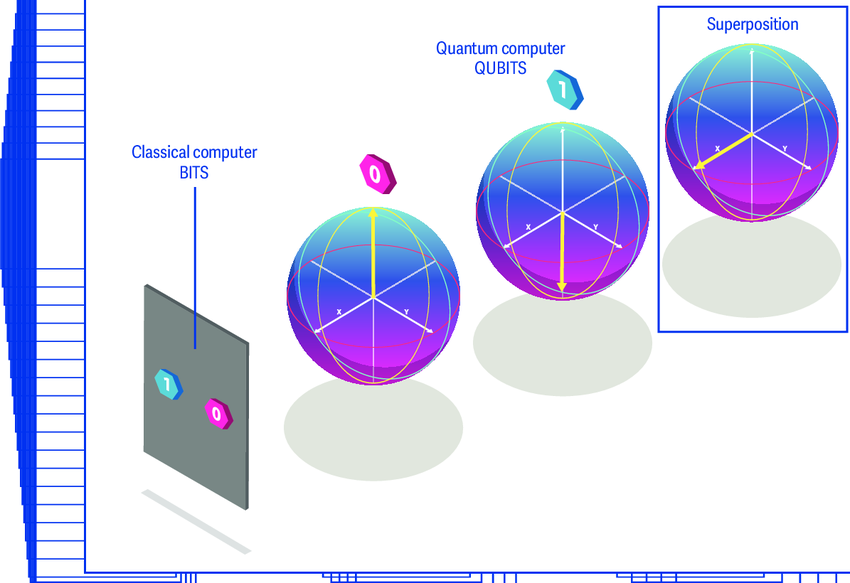
\includegraphics[width=0.7\textwidth]{quantum_vs_classical.png}
%    \caption{Comparison of Classical vs. Quantum Attack Complexity}
%    \label{fig:quantum_vs_classical}
%\end{figure}

\section{Shor's Algorithm}\label{sec:shors_algorithm}

Developed by Peter Shor in 1994 \parencite{shor1994algorithms}, Shor's algorithm is a landmark achievement. It demonstrates that quantum computers have the potential to factor large integers in polynomial time. This capability represents a serious threat to asymmetric cryptography, which depends on the computational difficulty of this very problem for its security \parencite{beckman1996efficient}.

The algorithm cleverly transforms the problem of factoring into one of finding the period of a function. Quantum computers can then efficiently determine this period using the quantum Fourier transform.

\begin{equation}\label{eq:shor_period}
    f(x) = a^x \bmod N
\end{equation}

where $N$ is the number to be factored and $a$ is a randomly chosen integer.

\begin{figure}[h]
    \centering
    \includegraphics[width=0.8\textwidth]{05_Quantum_Impact_on_Cryptography/shor_algorithm}
    \caption{Quantum circuit implementation of Shor's algorithm}
    \label{fig:shor_circuit}
\end{figure}

\section{Impact on RSA}\label{sec:rsa_impact}

The security of RSA depends on the difficulty of factoring:

\begin{equation}\label{eq:rsa_complexity}
    T_{\text{classical}} = O(e^{(\log N)^{1/3}(\log \log N)^{2/3}})
\end{equation}

Versus Shor's algorithm:
\begin{equation}\label{eq:shor_complexity}
    T_{\text{quantum}} = O((\log N)^2(\log \log N)(\log \log \log N))
\end{equation}

\section{Grover's Algorithm}\label{sec:grovers_algorithm}

While Shor's algorithm targets asymmetric cryptography, Grover's algorithm \parencite{grover1996fast} presents a different kind of challenge. It offers a quadratic speedup for unstructured search problems. What does this mean for cryptography?

\begin{itemize}
    \item \textbf{Symmetric Encryption:} Grover's algorithm effectively reduces the security of symmetric encryption by half. For example, AES-256 would become roughly equivalent in security to AES-128 against a quantum attacker \parencite{nist2001aes}.
    \item \textbf{Hash Functions:} Hash functions are similarly affected. Finding preimages or collisions becomes somewhat faster with Grover's algorithm.
    \item \textbf{The Solution: Key Size Increase:} To counteract Grover's algorithm, a straightforward approach is to double the key sizes for symmetric cryptography.
\end{itemize}

\begin{equation}\label{eq:grover_speedup}
    T_{\text{quantum}} = O(\sqrt{N})
\end{equation}

\begin{figure}[h]
    \centering
    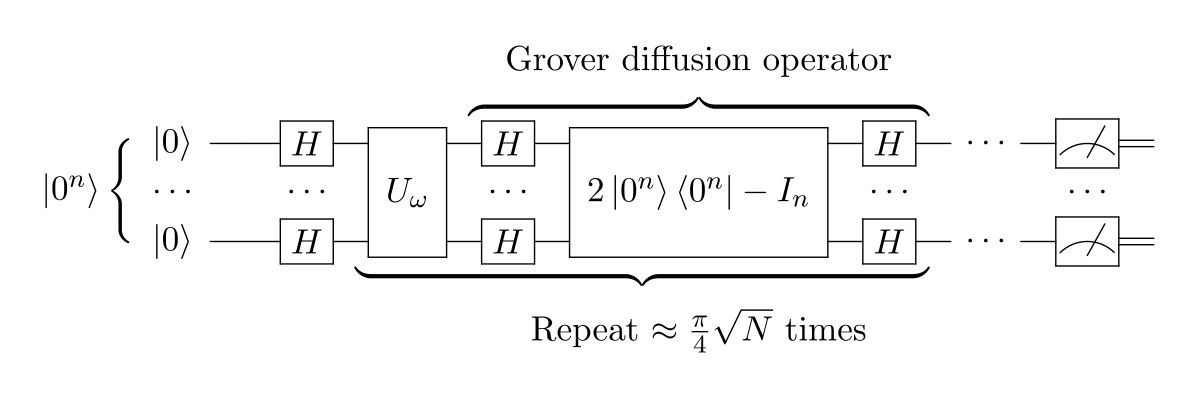
\includegraphics[width=0.8\textwidth]{05_Quantum_Impact_on_Cryptography/grovers_algorithm}
    \caption{Quantum circuit for Grover's algorithm}
    \label{fig:grover_circuit}
\end{figure}

\section{Timeline of Quantum Threat}\label{sec:timeline}

When might we expect quantum computers powerful enough to break current cryptography?  Estimates vary, but current thinking suggests that quantum computers capable of breaking RSA-2048 could potentially emerge within the next 5 to 15 years \parencite{mosca2018cybersecurity}.  However, significant hurdles remain:

\begin{itemize}
    \item \textbf{Error Correction:} Building quantum computers with sufficiently low error rates is a major technical challenge. Current error correction techniques are still imperfect \parencite{preskill2018quantum}.
    \item \textbf{Scalability:} Cryptographically relevant computations will likely require thousands of logical qubits. Scaling up current quantum computer prototypes to this size is a significant engineering undertaking.
\end{itemize}

\begin{figure}[h]
    \centering
    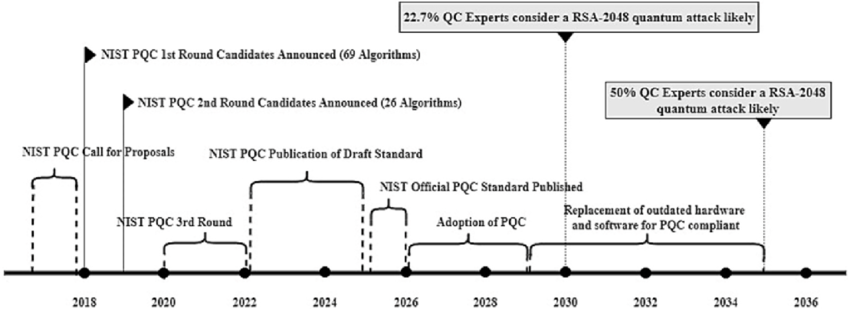
\includegraphics[width=0.8\textwidth]{06_Challenges_in_Transition/nist_timeline}
    \caption{NIST's projected timeline for quantum computer development}
    \label{fig:nist_timeline}
\end{figure}

\section{Store Now, Decrypt Later Attacks}

A significant near-term risk involves adversaries storing encrypted data now to decrypt it when quantum computers become available. This particularly threatens data with long-term value, making quantum-resistant solutions necessary even before practical quantum computers exist.

\section{Quantum-Resistant Algorithm Categories}
In response to quantum threats, cryptographers have developed several approaches to post-quantum cryptography:

\subsection{Lattice-Based Cryptography}
Lattice-based cryptosystems base their security on the hardness of certain problems in lattice theory, such as the Shortest Vector Problem (SVP) and the Learning With Errors (LWE) problem. These problems are believed to be difficult even for quantum computers. Notable examples include:
\begin{itemize}
    \item NTRU (N-th degree Truncated polynomial Ring Units)
    \item Kyber, a lattice-based key encapsulation mechanism selected by NIST for standardization
\end{itemize}

\subsection{Hash-Based Cryptography}
Hash-based signatures rely on the security of cryptographic hash functions, which are less vulnerable to quantum attacks. They include:
\begin{itemize}
    \item Merkle signature scheme
    \item XMSS (eXtended Merkle Signature Scheme), standardized by the IETF
    \item SPHINCS+, a stateless hash-based signature scheme selected by NIST
\end{itemize}

\subsection{Code-Based Cryptography}
Code-based cryptography uses error-correcting codes and derives its security from the difficulty of decoding general linear codes. McEliece, proposed in 1978, is one of the oldest post-quantum cryptographic systems and has withstood decades of cryptanalysis.

\subsection{Multivariate Polynomial Cryptography}
These systems base their security on the difficulty of solving systems of multivariate polynomials over finite fields, known to be NP-hard. Examples include the Rainbow signature scheme, though recent cryptanalysis has identified vulnerabilities in some variants.

\subsection{Isogeny-Based Cryptography}
Isogeny-based systems rely on the difficulty of finding isogenies between elliptic curves. SIKE (Supersingular Isogeny Key Encapsulation) was a notable example, though it was subsequently broken by classical attacks in 2022, highlighting the evolving nature of post-quantum cryptography research.

\section{Standardization Efforts}
The transition to quantum-resistant cryptography requires coordinated standardization efforts:

\subsection{NIST Post-Quantum Cryptography Standardization}
The U.S. National Institute of Standards and Technology launched its post-quantum cryptography standardization process in 2016. After multiple rounds of evaluation, NIST selected several algorithms for standardization in 2022:
\begin{itemize}
    \item For key encapsulation: CRYSTALS-Kyber
    \item For digital signatures: CRYSTALS-Dilithium, FALCON, and SPHINCS+
\end{itemize}

Final standards are expected to be published by 2024-2025, with additional algorithms still under consideration for future standardization.

\subsection{Other Standardization Bodies}
In parallel with NIST, other organizations are contributing to post-quantum standardization:
\begin{itemize}
    \item The Internet Engineering Task Force (IETF) is developing protocols for incorporating post-quantum algorithms into TLS and other internet standards
    \item The European Telecommunications Standards Institute (ETSI) has established a Quantum-Safe Cryptography working group
    \item The International Organization for Standardization (ISO) is developing standards for quantum-resistant cryptographic techniques
\end{itemize}

\section{Transition Challenges}
Migrating from classical to post-quantum cryptography presents significant challenges:

\subsection{Computational and Bandwidth Overhead}
Most post-quantum algorithms require larger key sizes and ciphertexts than their classical counterparts, imposing:
\begin{itemize}
    \item Increased computational demands on both servers and clients
    \item Higher bandwidth requirements for communication protocols
    \item Storage challenges for certificates and cryptographic artifacts
\end{itemize}

\subsection{Implementation and Deployment Considerations}
The transition process involves numerous practical considerations:
\begin{itemize}
    \item Identifying all systems using vulnerable cryptography
    \item Prioritizing critical infrastructure and long-term secrets
    \item Developing migration strategies that maintain backward compatibility
    \item Implementing hybrid approaches that combine classical and post-quantum algorithms during the transition period
\end{itemize}

\subsection{Cryptographic Agility}
A key lesson from the quantum threat is the importance of building cryptographic agility into systems—the ability to quickly replace cryptographic algorithms without major system overhauls. This approach provides resilience against future cryptographic vulnerabilities, whether quantum-related or otherwise.

\section{Current Industry Responses}
Major technology companies and organizations have already begun implementing quantum-resistant approaches:
\begin{itemize}
    \item Google has tested post-quantum algorithms in Chrome and other products
    \item Cloudflare has implemented experimental support for post-quantum TLS
    \item Microsoft has developed quantum-resistant VPN solutions
    \item Financial institutions are evaluating the impact on banking infrastructure and payment systems
    \item Military and intelligence agencies worldwide are prioritizing quantum-resistant encryption for classified communications
\end{itemize}

These early adoption efforts provide valuable real-world testing for post-quantum algorithms while protecting particularly sensitive systems against future quantum threats.

\section{Comparative Analysis}\label{sec:comparison}

\begin{table}[h]
    \centering
    \caption{Impact of Quantum Computing on Classical Cryptography}
    \label{tab:quantum_impact}
    \begin{tabular}{|l|c|c|}
        \hline
        \textbf{Algorithm} & \textbf{Classical Security} & \textbf{Quantum Security} \\
        \hline
        RSA-2048 & 112 bits & 0 bits \\
        AES-256 & 256 bits & 128 bits \\
        ECC-256 & 128 bits & 0 bits \\
        \hline
    \end{tabular}
\end{table}

\section{Required Security Levels}\label{sec:security_levels}

To maintain security against quantum attacks:

\begin{itemize}
    \item \textbf{Symmetric Key Algorithms:} Double the key length
    \item \textbf{Hash Functions:} Double the output length
    \item \textbf{Public Key Algorithms:} Replace with quantum-resistant alternatives
\end{itemize}

The required security level $S$ against quantum attacks is:
\begin{equation}\label{eq:quantum_security}
    S_{\text{quantum}} = \frac{S_{\text{classical}}}{2}
\end{equation}

This chapter demonstrates the urgent need for quantum-resistant cryptography, which we will explore in subsequent chapters.